\documentclass{standalone}

\usepackage{fontspec}
\setmainfont{osifont.ttf}
\fontsize{3.5mm}{4mm}\selectfont

\newcommand\formatname{A4}

\usepackage{tikz}

\begin{document}
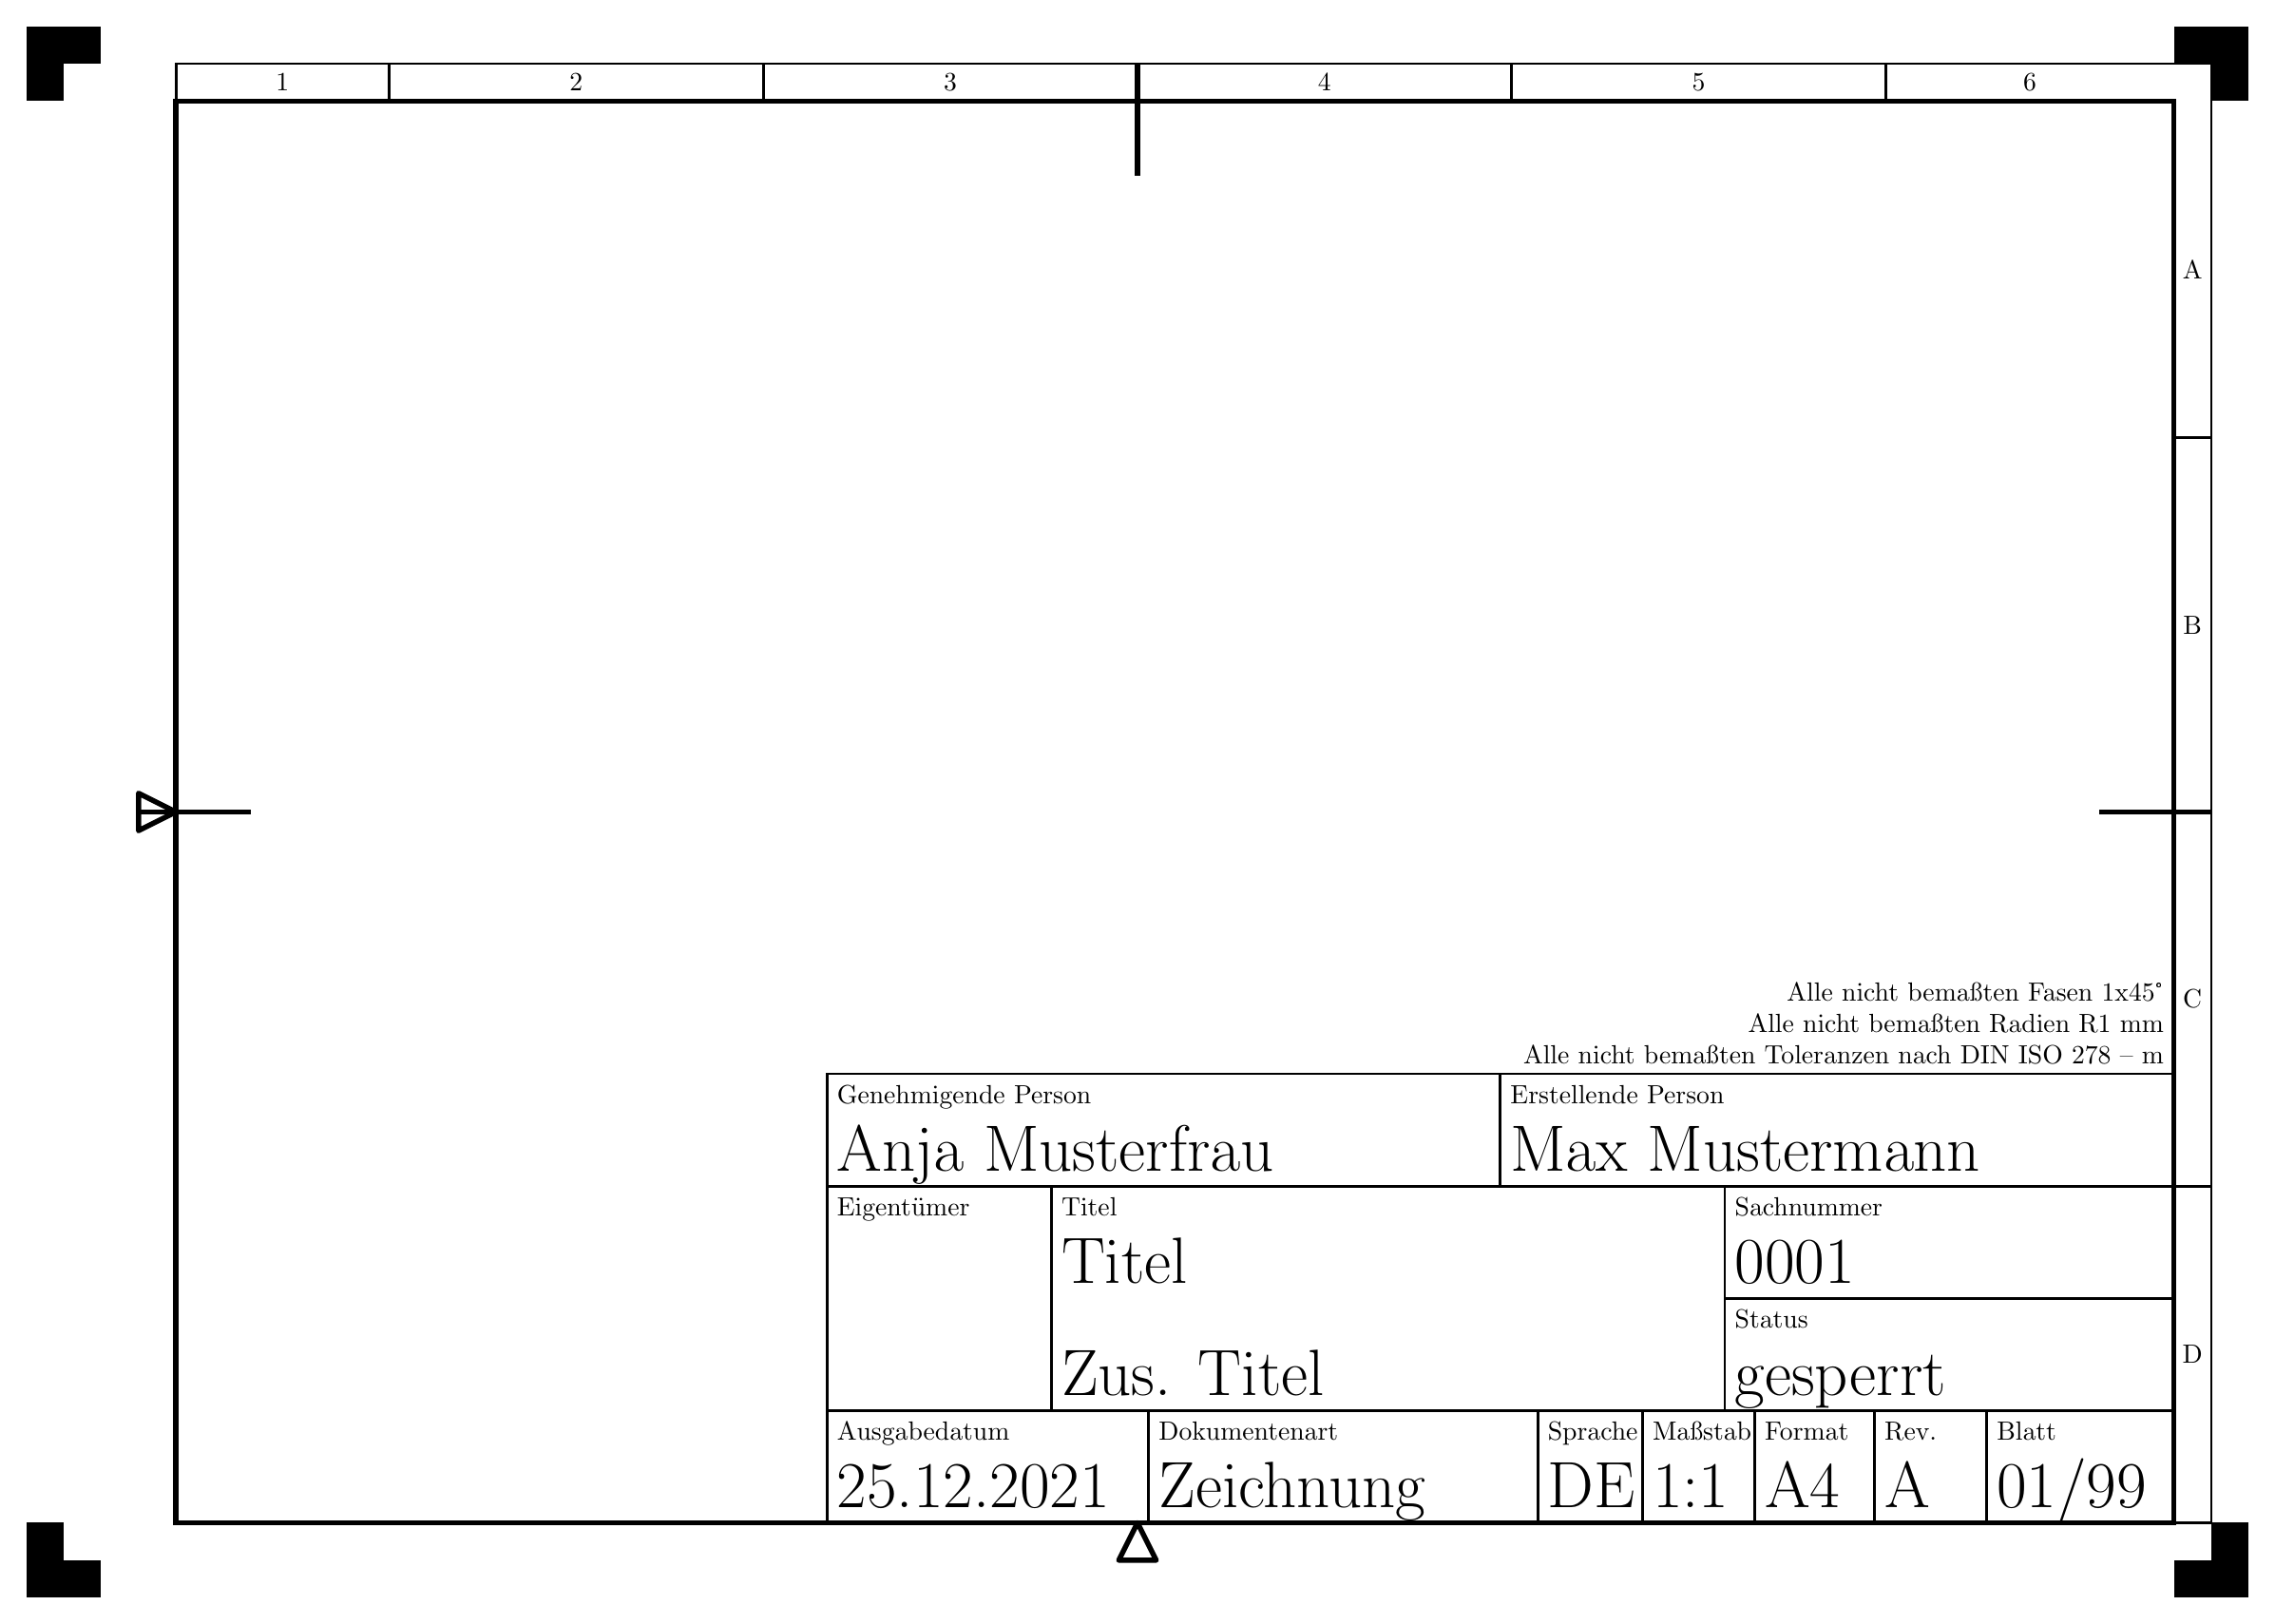
\begin{tikzpicture}[yscale = -1, line width = 0.35mm]
	\fill (0, 0) rectangle (10mm, 5mm);
	\fill (0, 0) rectangle (5mm, 10mm);
	\fill (297mm, 0) rectangle (287mm, 5mm);
	\fill (297mm, 0) rectangle (292mm, 10mm);
	\fill (0, 210mm) rectangle (10mm, 205mm);
	\fill (0, 210mm) rectangle (5mm, 200mm);
	\fill (297mm, 210mm) rectangle (287mm, 205mm);
	\fill (297mm, 210mm) rectangle (292mm, 200mm);

	% Zeichenbereich:
	\draw [line width = 0.7mm] (20mm, 10mm) rectangle (287mm, 200mm);

	% Mittellinien:
	\begin{scope}[line width = 0.7mm, line join = round]
		\draw (15mm, 105mm) -- (30mm, 105mm);
		\draw (292mm, 105mm) -- (277mm, 105mm);
		\draw (148.5mm, 5mm) -- (148.5mm, 20mm);
		%\draw (148.5mm, 205mm) -- (148.5mm, 190mm);
		
		% Mittellinien ohne Feldeinteilung:
		\draw (20mm, 105mm) -- (15mm, 102.5mm) -- (15mm, 107.5mm) -- cycle;
		\draw (148.5mm, 200mm) -- (146mm, 205mm) -- (151mm, 205mm) -- cycle;
	\end{scope}

	%Feldeinteilung
	\draw (20mm, 5mm) rectangle (292mm, 200mm);
	\foreach \y in {55mm, 155mm} {
		\draw (287mm, \y) -- (292mm, \y);
	}
	\node at (289.5mm, 32.5mm) {A};
	\node at (289.5mm, 80mm) {B};
	\node at (289.5mm, 130mm) {C};
	\node at (289.5mm, 177.5mm) {D};
	
	\foreach \x in {48.5mm, 98.5mm, 198.5mm, 248.5mm} {
		\draw (\x, 5mm) -- (\x, 10mm);
	}
	\node at (34.25mm, 7.5mm) {1};
	\node at (73.5mm, 7.5mm) {2};
	\node at (123.5mm, 7.5mm) {3};
	\node at (173.5mm, 7.5mm) {4};
	\node at (223.5mm, 7.5mm) {5};
	\node at (267.75mm, 7.5mm) {6};

	% Schriftfeld
	\draw (287mm, 200mm) rectangle (107mm, 140mm);

	\begin{scope}[anchor = base west, xshift = 107mm, yshift = 140mm]
		% Zeilen
\draw (0mm, 15mm) -- (180mm, 15mm);
\draw (0mm, 45mm) -- (180mm, 45mm);

% Zeile 1
\node at (0mm, 4mm) {Genehmigende Person};
\node at (0mm, 13mm) {\fontsize{10mm}{11mm}\selectfont Anja Musterfrau};
\node at (90mm, 4mm) {Erstellende Person};
\node at (90mm, 13mm) {\fontsize{10mm}{11mm}\selectfont Max Mustermann};
\foreach \x in {90mm} {
	\draw (\x, 0mm) -- (\x, 15mm);
}

% Zeile 2
\node at (0mm, 19mm) {Eigentümer};
\node at (30mm, 19mm) {Titel};
\node at (30mm, 28mm) {\fontsize{10mm}{11mm}\selectfont Titel};
\node at (30mm, 43mm) {\fontsize{10mm}{11mm}\selectfont Zus. Titel};
\foreach \x in {30mm, 120mm} {
	\draw (\x, 15mm) -- (\x, 45mm);
}
\draw (120mm, 30mm) -- (180mm, 30mm);
\node at (120mm, 19mm) {Sachnummer};
\node at (120mm, 28mm) {\fontsize{10mm}{11mm}\selectfont 0001};
\node at (120mm, 34mm) {Status};
\node at (120mm, 43mm) {\fontsize{10mm}{11mm}\selectfont gesperrt};

% Zeile 3
\node at (0mm, 49mm) {Ausgabedatum};
\node at (0mm, 58mm) {\fontsize{10mm}{11mm}\selectfont 25.12.2021};
\node at (43mm, 49mm) {Dokumentenart};
\node at (43mm, 58mm) {\fontsize{10mm}{11mm}\selectfont Zeichnung};
\node at (95mm, 49mm) {Sprache};
\node at (95mm, 58mm) {\fontsize{10mm}{11mm}\selectfont DE};
\node at (109mm, 49mm) {Maßstab};
\node at (109mm, 58mm) {\fontsize{10mm}{11mm}\selectfont 1:1};
\node at (124mm, 49mm) {Format};
\node at (124mm, 58mm) {\fontsize{10mm}{11mm}\selectfont \formatname};
\node at (140mm, 49mm) {Rev.};
\node at (140mm, 58mm) {\fontsize{10mm}{11mm}\selectfont A};
\node at (155mm, 49mm) {Blatt};
\node at (155mm, 58mm) {\fontsize{10mm}{11mm}\selectfont 01/99};
\foreach \x in {43mm, 95mm, 109mm, 124mm, 140mm, 155mm} {
	\draw (\x, 45mm) -- (\x, 60mm);
}

	\end{scope}

	% Weitere Hinweise
	\begin{scope}[anchor = south east]
		\node [align = right] at (287mm, 140mm) {Alle nicht bemaßten Fasen 1x45°\\Alle nicht bemaßten Radien R1 mm\\Alle nicht bemaßten Toleranzen nach DIN ISO 278 -- m};
	\end{scope}
\end{tikzpicture}
\end{document}
